\renewcommand{\arraystretch}{0.6}
\section{Halbleiter}
\begin{itemize}
    \item \textbf{Metallische Leiter:} der Stromtransport wird durch Elektronen erzeugt.
    \item \textbf{Isolatoren:} der Stromtransport wird durch Isolatoren erzeugt.
    \item \textbf{Halbleiter:} die Leitfähigkeit liegt irgendwo zwischen Metallen und Isolatoren.
    \subitem  Die wichtigsten Halbleiter sind  Si, Ge, $CuO_2$ und GaAs 
    \item \textbf{Dotierte Halbleiter:} Durch kontrollierte Verunreinigung (Dotierung) der reinen Halbleiterwerkstoffe kann die Leitfähigkeit wesentlich verändert werden.
\end{itemize}
\subsection{Kristallgitter} 
\begin{minipage}{\linewidth}
        \begin{wrapfigure}{r}{4cm}
            \vspace{-1cm}
            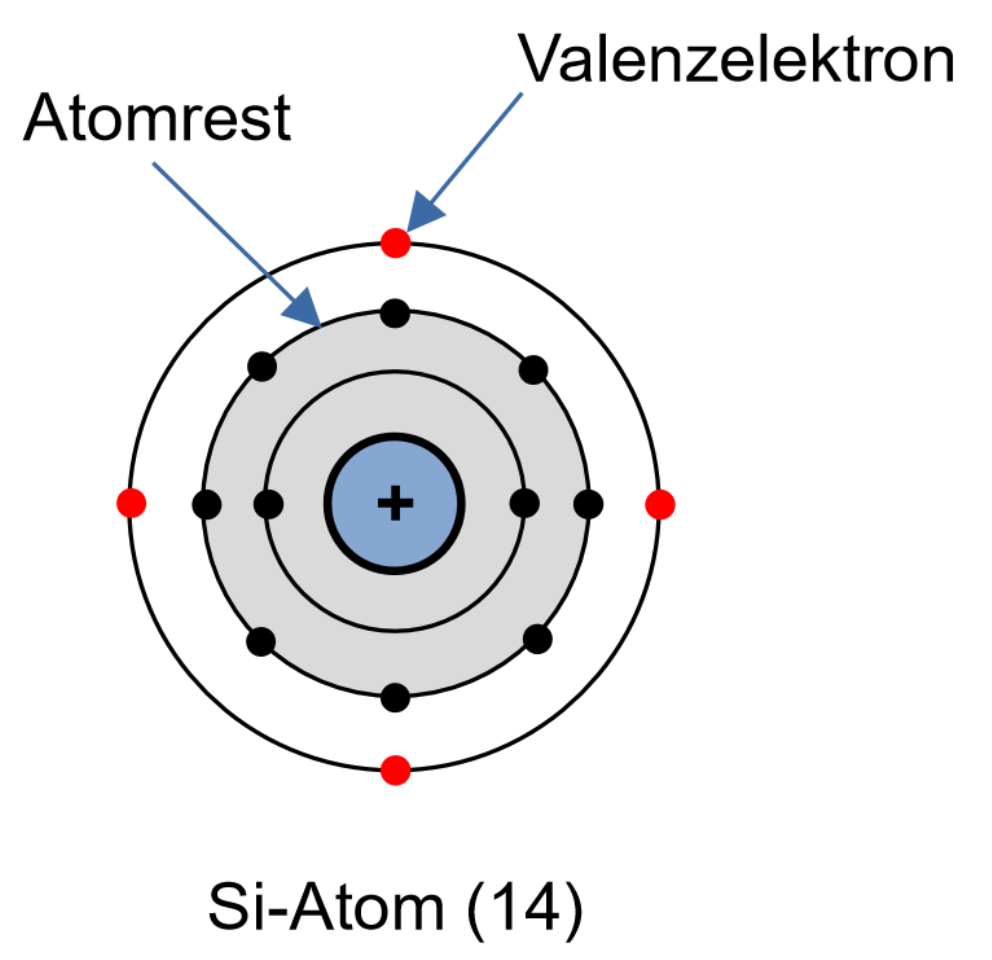
\includegraphics[width=\linewidth]{images/Si-Atom14}  
        \end{wrapfigure}
    Durch die thermische Bewegung der Atomem um ihre Ruhelage im Kristallgitter ist es möglich einige \textbf{Elektronenpaarbindungen} aufzubrechen.\newline
    Auf diese weise ein gelöstes Elektron bewegt sich im Kristallgitter frei und hinterlässt eine \textbf{positiv geladene Lücke im Kristallgitter} (Defektelektron)
\end{minipage}
\newline
\hspace{2cm}
\begin{minipage}{0.3\linewidth}
    \hspace{2cm}
    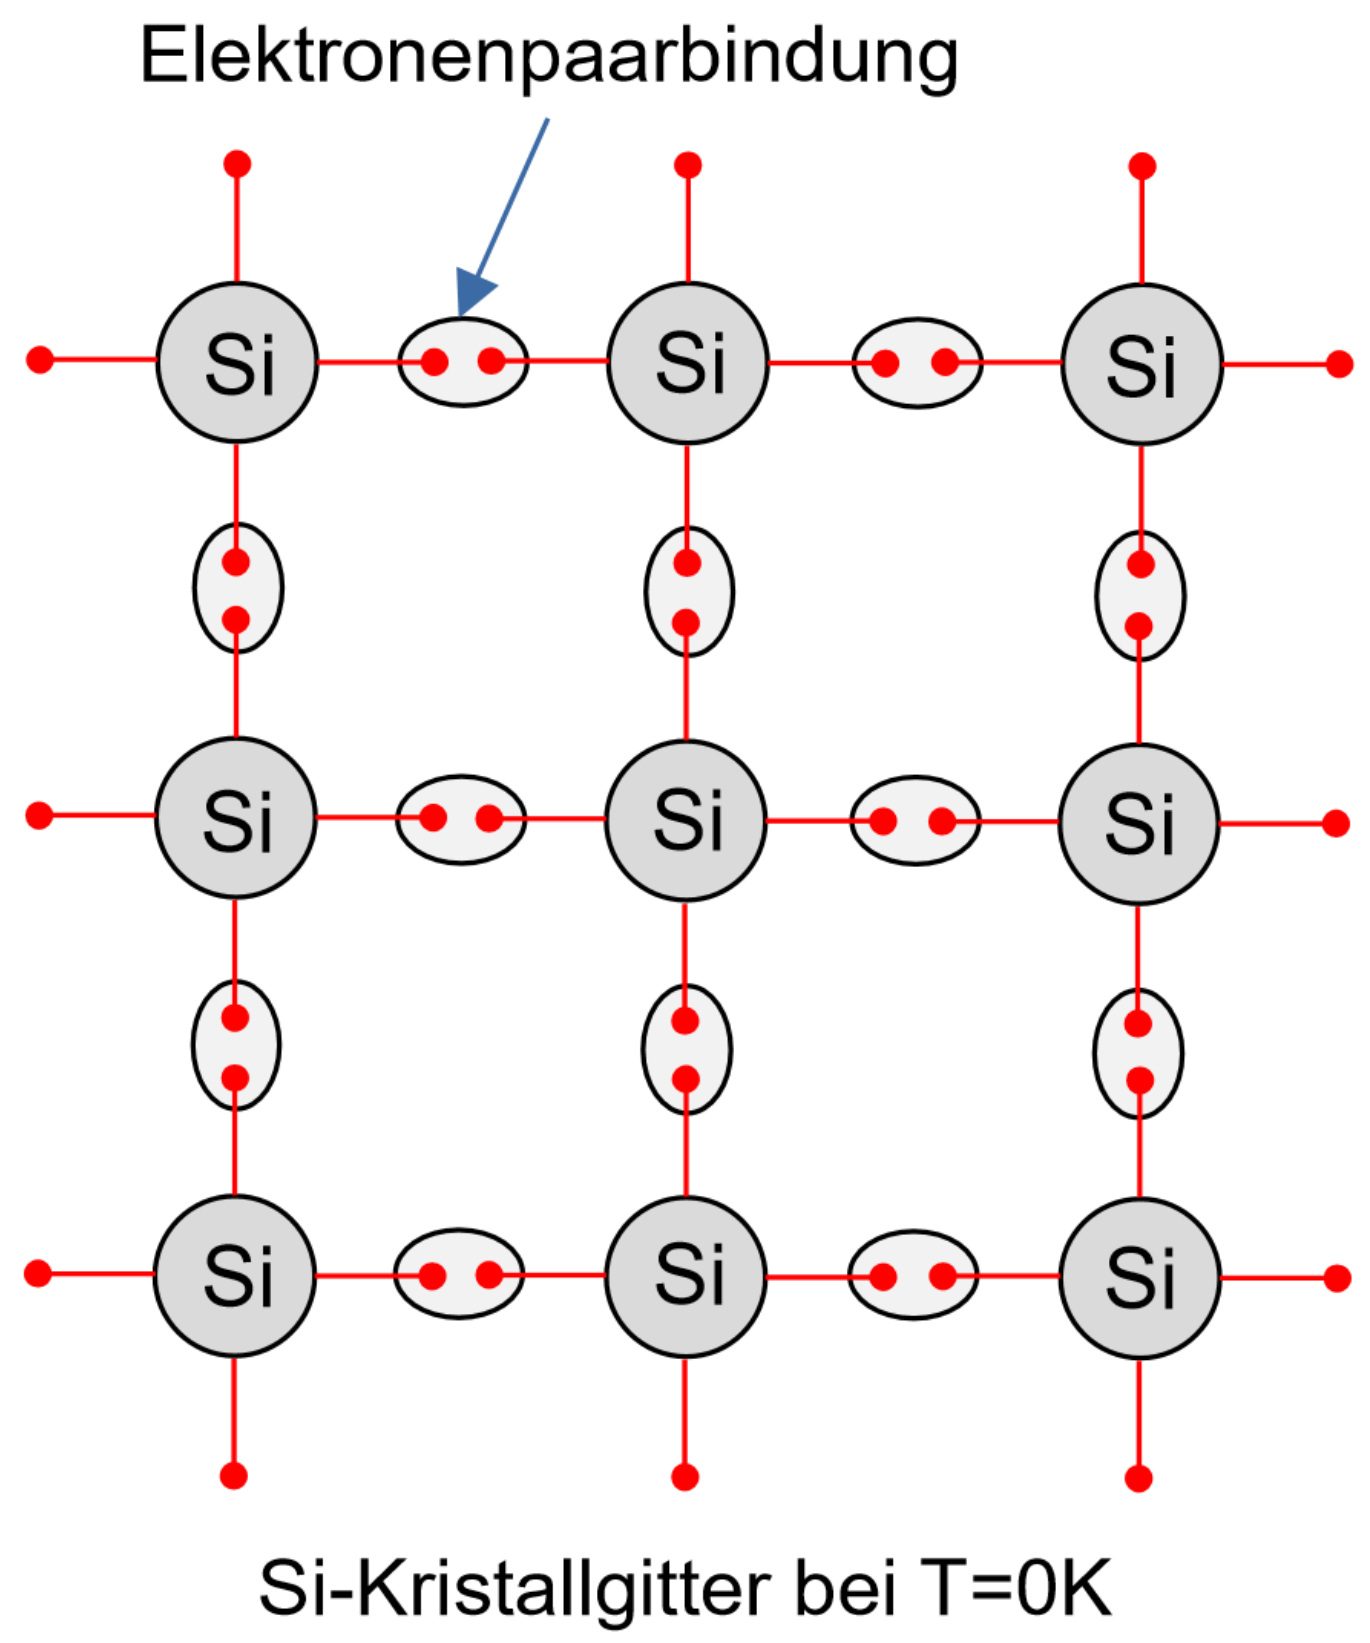
\includegraphics[width=0.8\linewidth]{images/RGSiT0K}
\end{minipage}
\hspace{2cm}
\begin{minipage}{0.3\linewidth}
    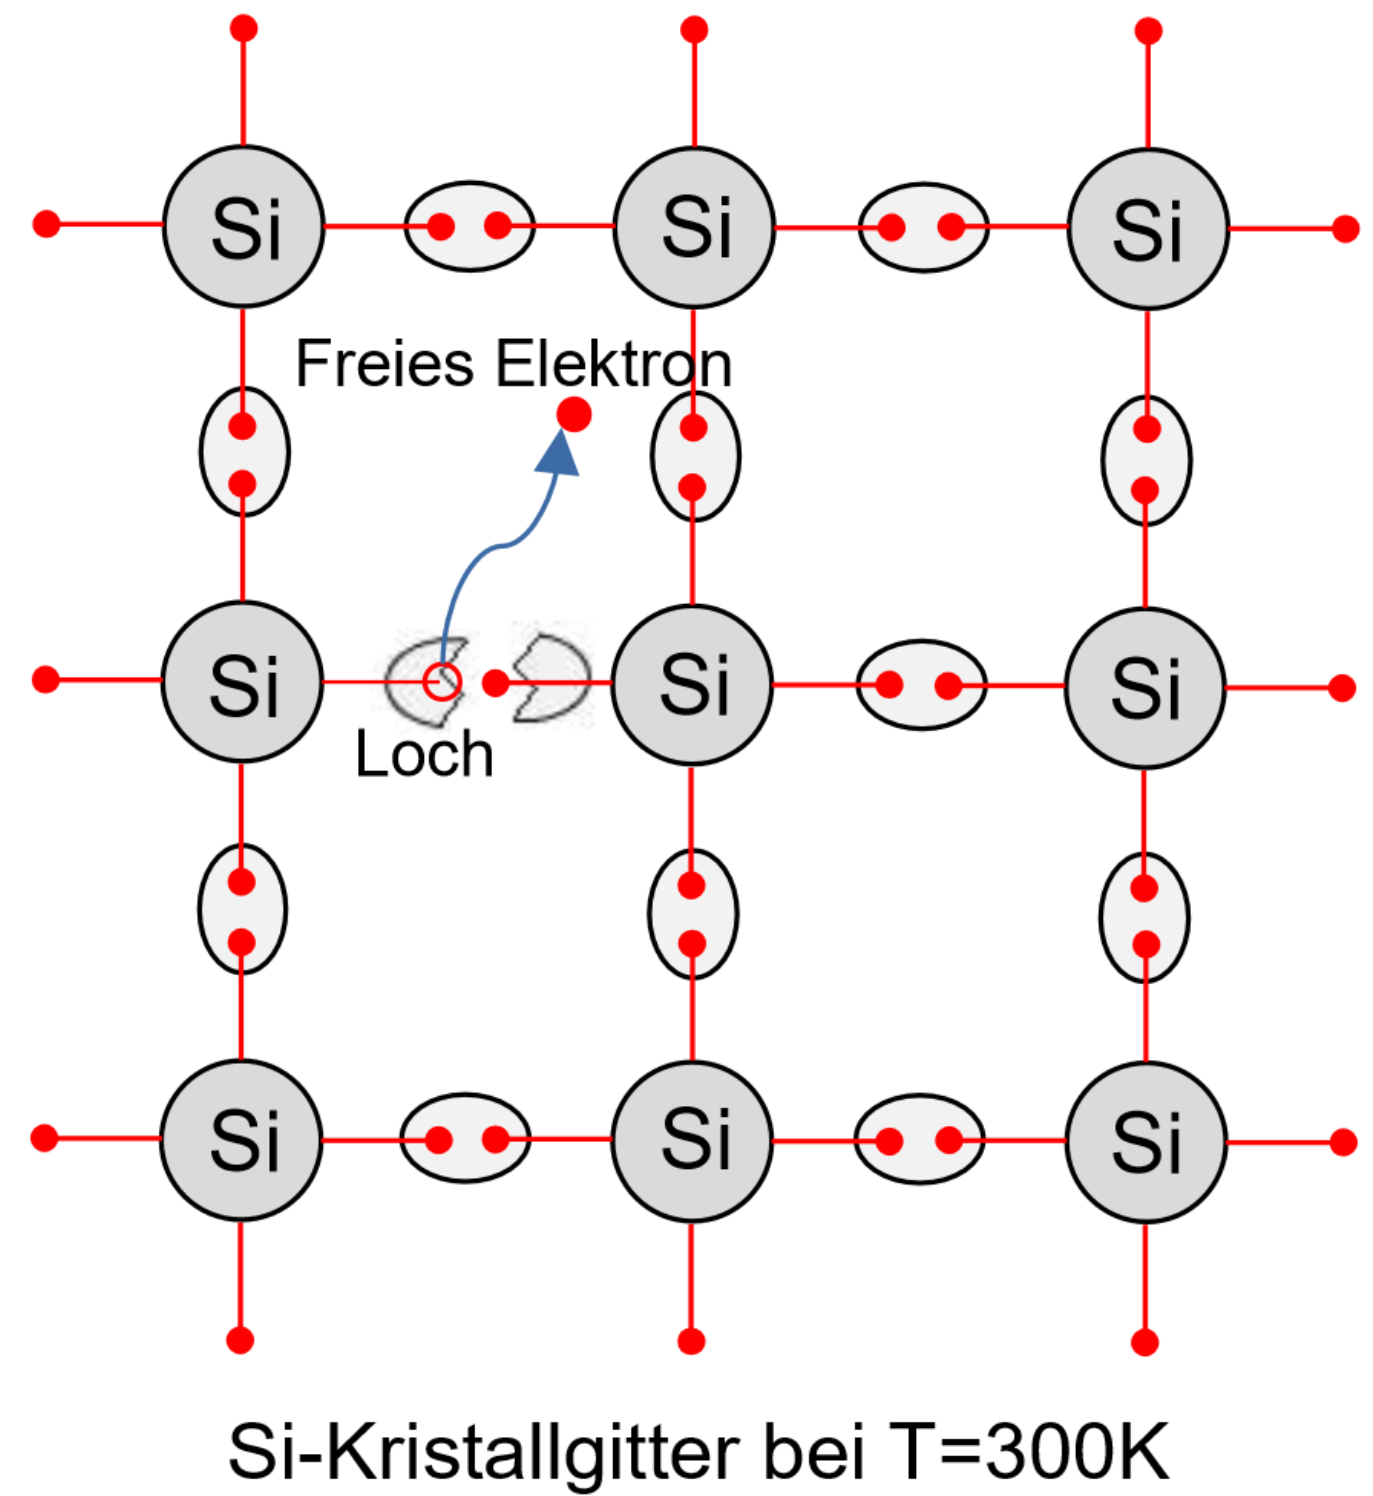
\includegraphics[width=0.8\linewidth]{images/RGSiT300K} 
\end{minipage}
    
\begin{multicols}{2}
\begin{minipage}{\linewidth}
    \subsection{Dotierung}
   Durch eine Dotierung des Halbleitermaterials mit Fremdatomen ist es möglich die Ladungsträgerdichte effizient zu kontrollieren:
\end{minipage}
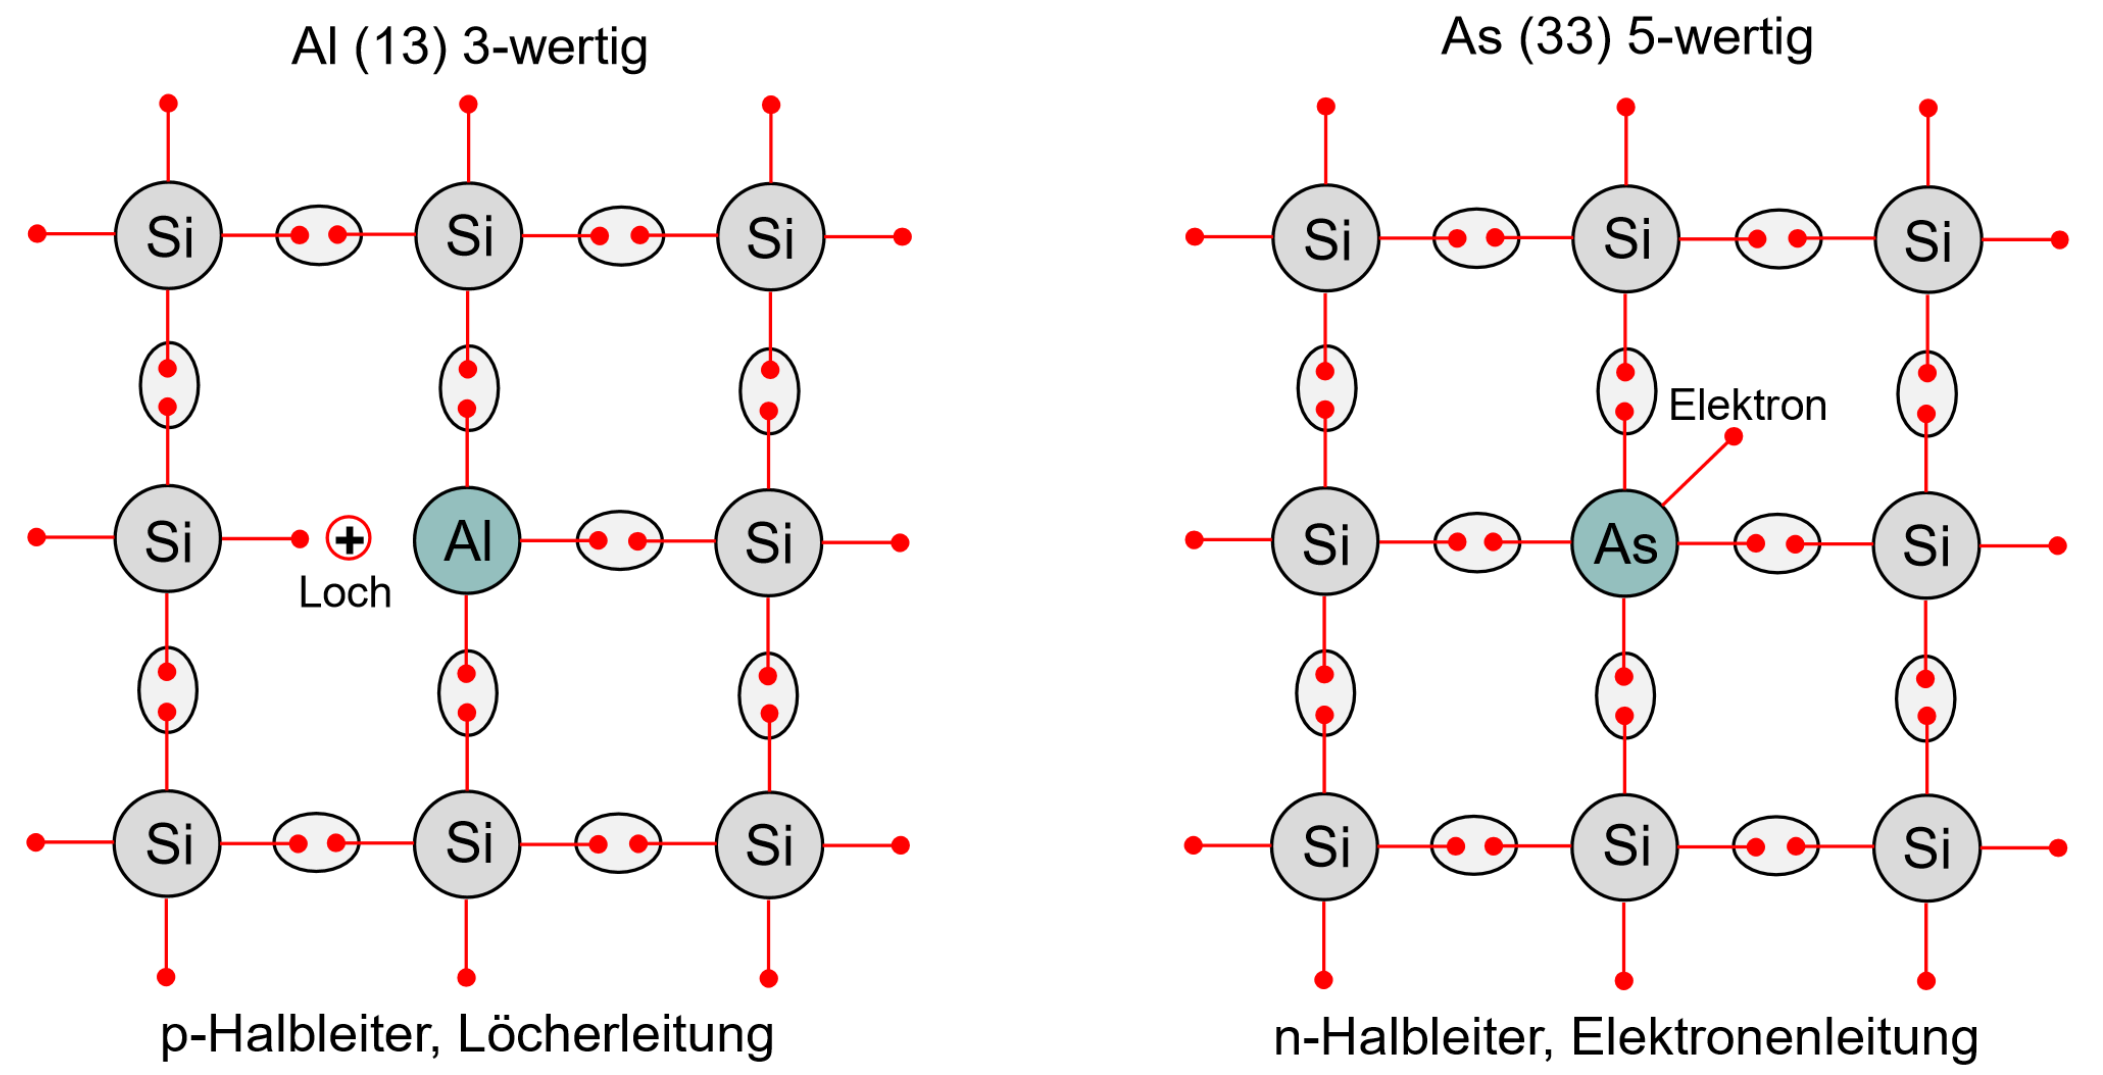
\includegraphics[width=0.8\linewidth]{images/SiAsDotierung}
\end{multicols}

\begin{multicols}{2}
    \begin{minipage}{\linewidth}
        \vspace{-2cm}
        \subsection{pn-Übergang}
        \subsubsection{Diffusionsstrom}
            Der Diffusionsstrom wird durch den Ladungsträgeraustausch zwischen beiden Halbleitergebieten erzeugt und dadurch verschwinden in der Grenzschicht alle freien Ladungsträger.\\
            Durch die Elektronenwanderung entsteht im n-Teil des Grenzgebiets die \textbf{ortsfeste} Positive Ladung(+). Die eindiffundierten Elektronen erzeugen im p-Teil des Grenzgebiets die \textbf{ortsfeste} negative Ladung (-). Die ortsfesten Ladungen erzeugen das elektrische Feld in der Raumladungszone und dammit auch den Driftstrom.\newline
            Der Driftstrom ist gegen den Diffusionsstrom gerichtet. Sobald die Ströme gleich sind, ist eine stabile Raumladungszone etabliert.   
    \end{minipage}
    
    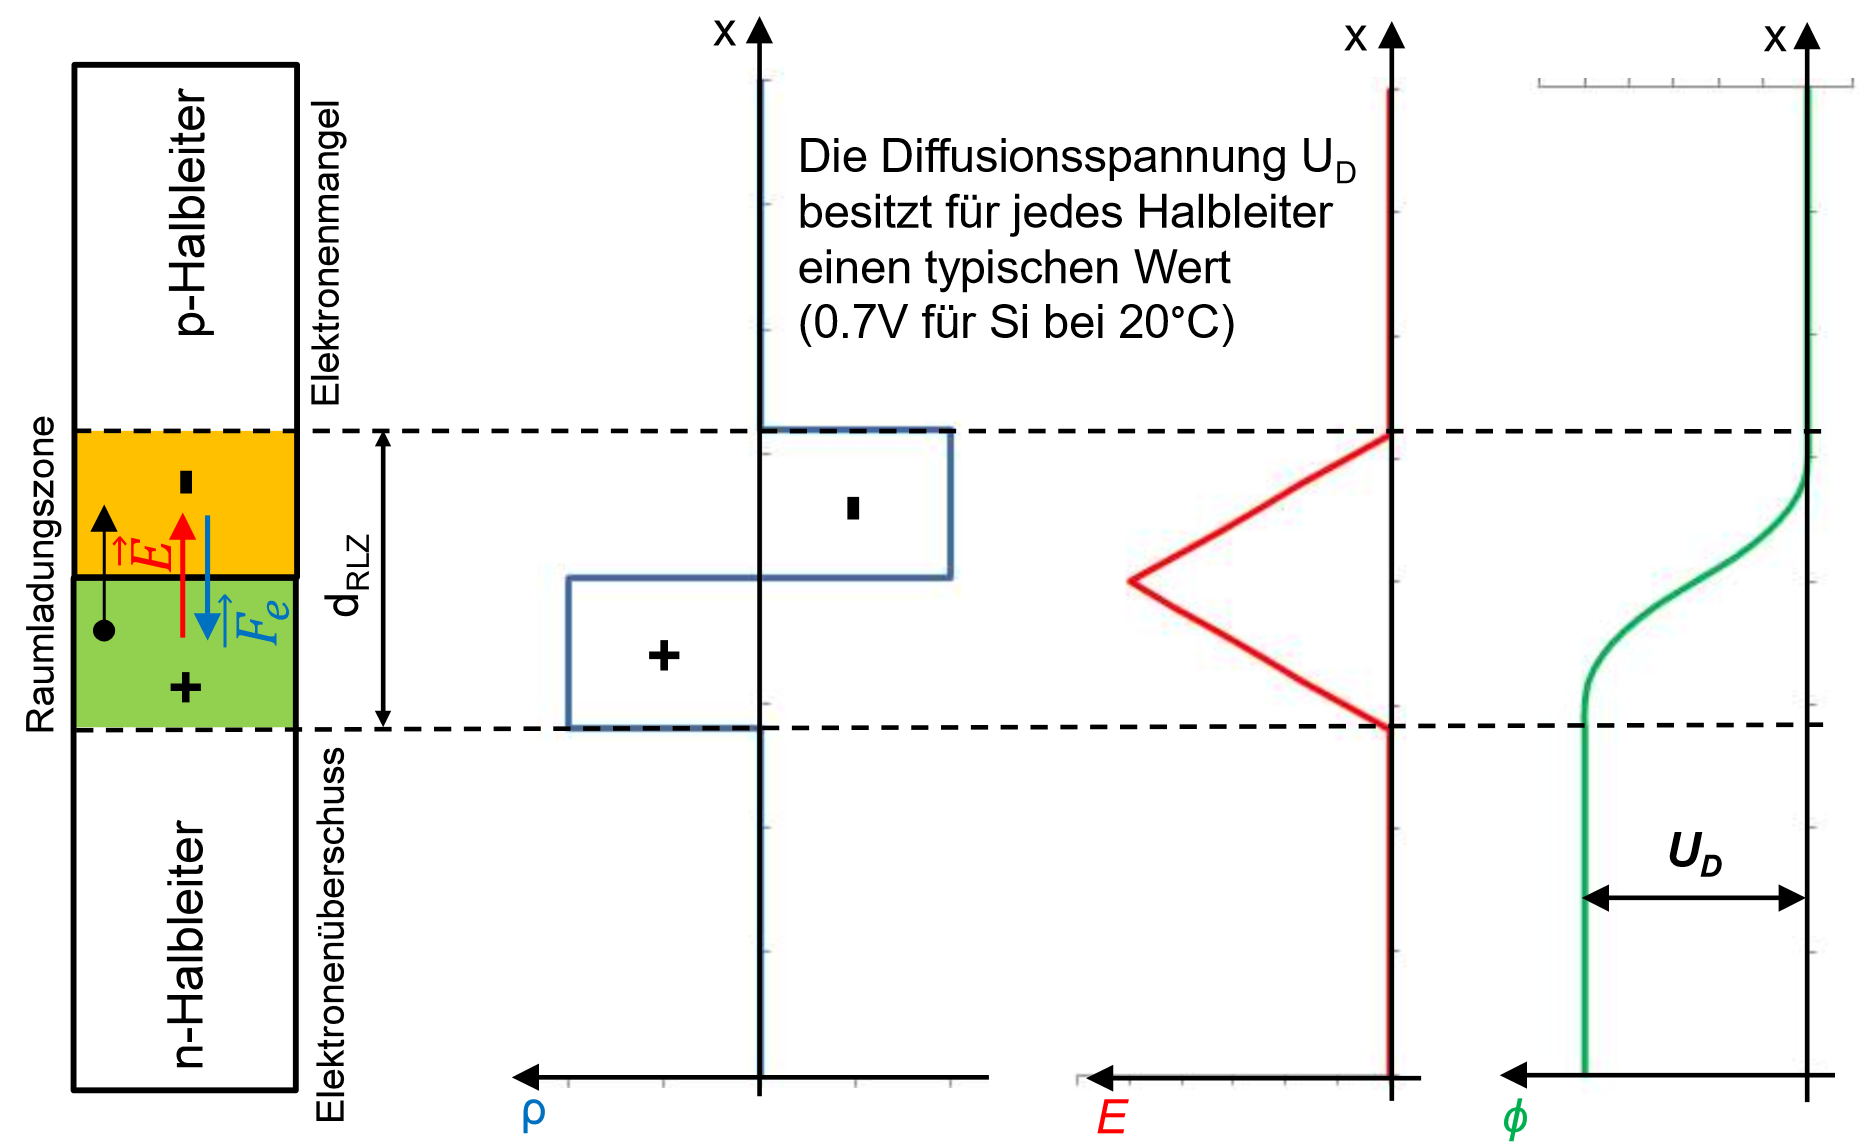
\includegraphics[width=0.9\linewidth]{images/pnuebergang}
\end{multicols}

\begin{minipage}{\linewidth}
        \subsubsection{pn-Übergang mit äusserer Spannung}
    \begin{wrapfigure}{r}{5cm}
       \vspace{-1cm}
        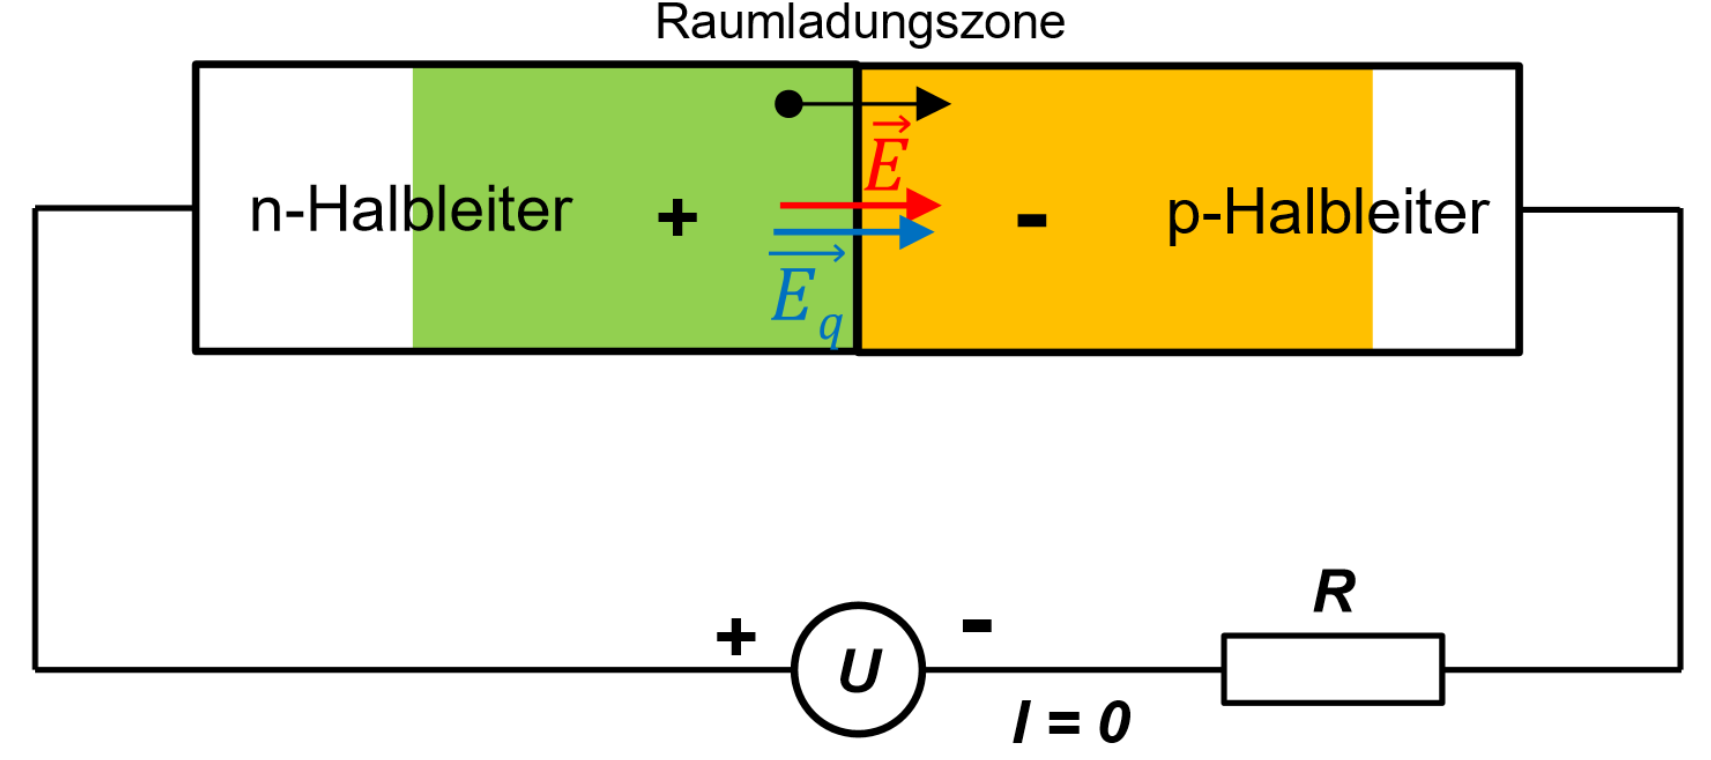
\includegraphics[width=\linewidth]{images/pnuebergengmitu}
    \end{wrapfigure}
    Die Spannungsquelle ist an den pn-Übergang in \textbf{Sperrrichtung} geschalten.\newline
    Die Spannung U vergrössert die Breite der Raumladungszone. Der Strom kann nicht über den pn-Übergang fliessen.
\end{minipage}
%TODO übersicht silizium germanium selen vor und nachteile
\clearpage